\documentclass[border=10pt]{standalone}
% Shared preamble for the README figures. Build with `docs/figures/build.sh`.
\usepackage[T1]{fontenc}
\usepackage{libertinus}
\setmonofont{Inconsolatazi4-Regular.otf}[Scale=0.86,BoldFont=Inconsolatazi4-Bold.otf]
\usepackage{amsmath}
\usepackage{tikz}
\usepackage{pgfplots}
\pgfplotsset{compat=1.18}
\usetikzlibrary{arrows.meta,positioning,calc,fit,backgrounds,decorations.pathreplacing,shapes.geometric,patterns}

\definecolor{ink}{gray}{0.11}
\definecolor{mute}{gray}{0.40}
\definecolor{faint}{gray}{0.62}
\definecolor{rule}{gray}{0.80}
\definecolor{fill}{gray}{0.955}
\definecolor{neg}{RGB}{164,38,44}
\definecolor{negfill}{RGB}{247,229,228}
\pagecolor{white}
\color{ink}

\tikzset{
  >={Stealth[length=5pt,width=4pt]},
  every picture/.style={line width=0.55pt, draw=ink},
  panel/.style={draw=rule, line width=0.6pt, fill=white},
  box/.style={draw=ink, fill=white, inner sep=3pt, font=\footnotesize},
  soft/.style={draw=rule, fill=fill, inner sep=3pt, font=\footnotesize},
  lab/.style={font=\footnotesize\color{mute}, inner sep=0pt},
  flow/.style={->, draw=ink, line width=0.7pt},
  code/.style={draw=rule, fill=fill, align=left, inner sep=4pt, font=\ttfamily\scriptsize, execute at begin node={\hyphenpenalty=10000\relax\exhyphenpenalty=10000\relax}},
}
\newcommand{\plabel}[2]{\textbf{(#1)}\,\textsc{#2}}

\begin{document}
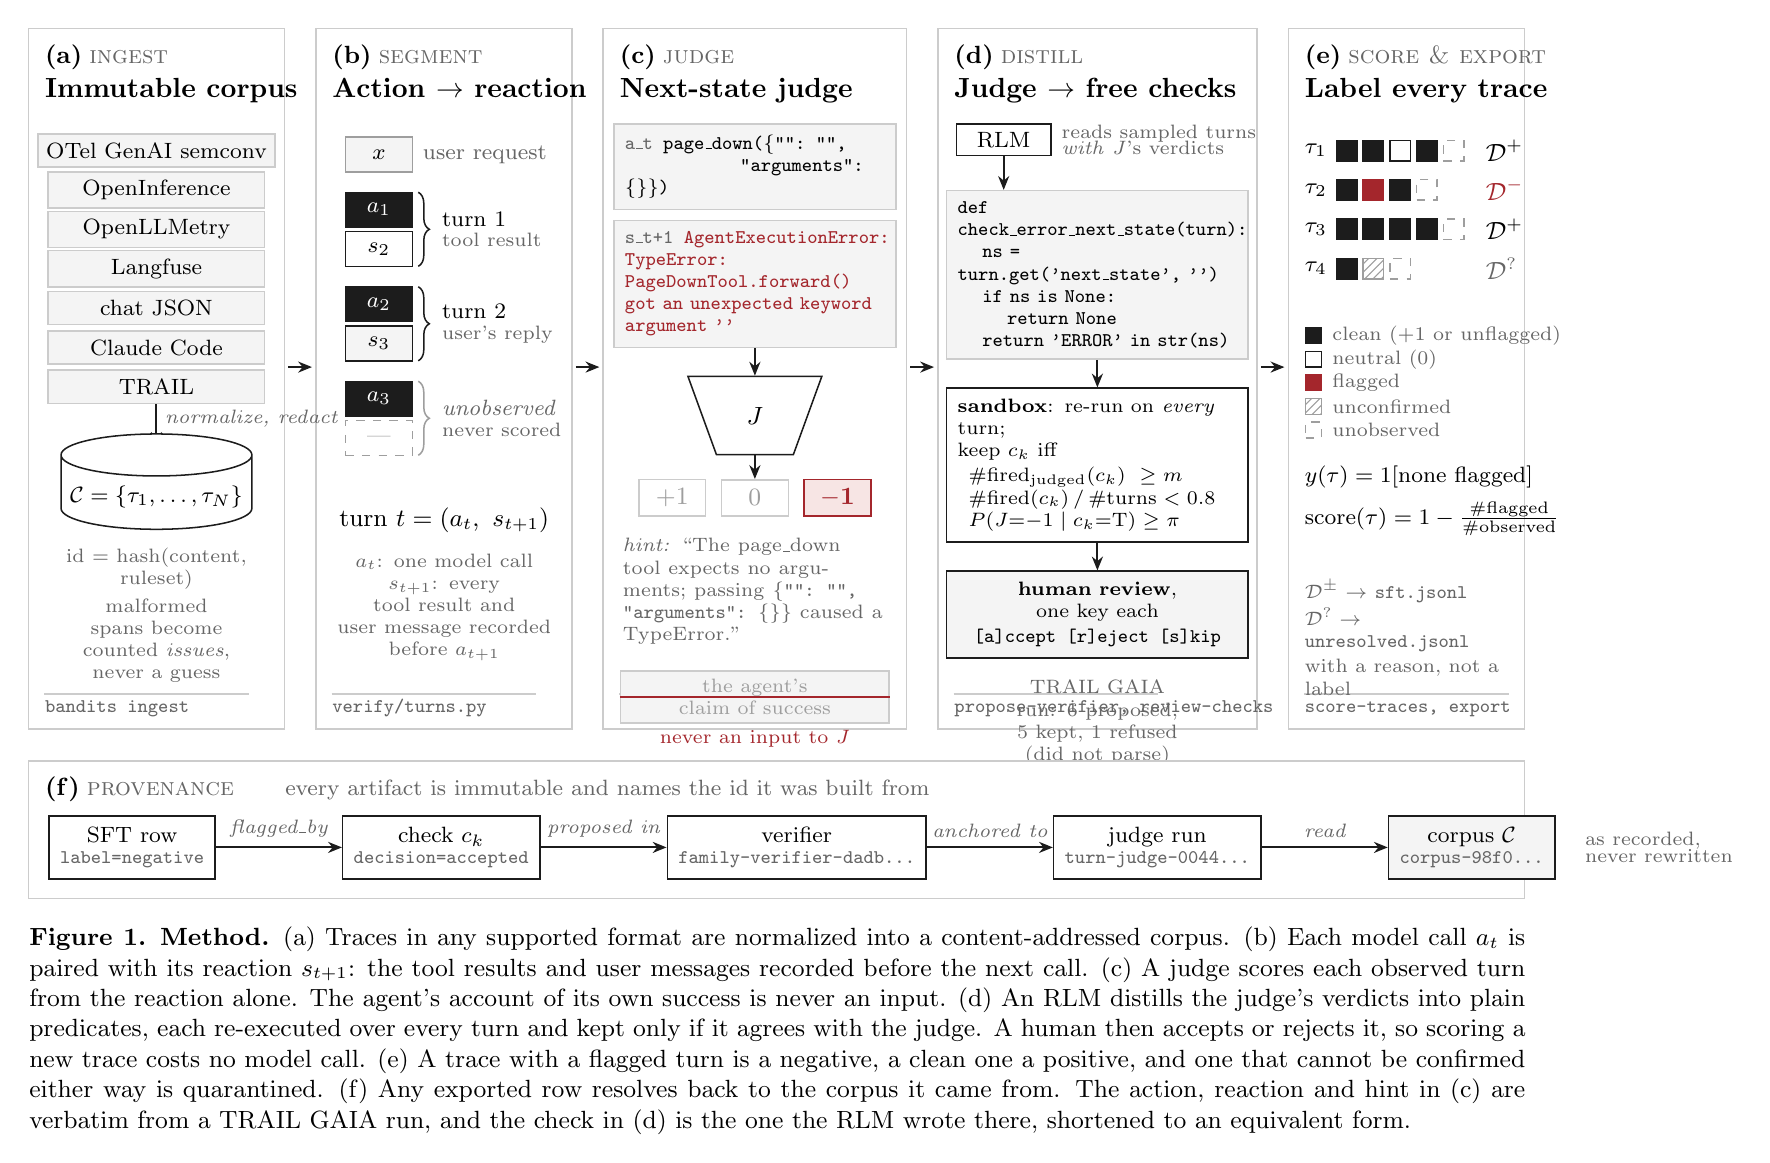
\begin{tikzpicture}[x=1cm,y=1cm]

% ---------- panel frames ----------
\def\bot{-8.9}
\foreach \name/\x/\w in {a/0/3.25, b/3.65/3.25, c/7.30/3.85, d/11.55/4.05, e/16.00/3.00}{
  \draw[panel] (\x,0) rectangle ++(\w,\bot);
  \coordinate (\name-nw) at (\x,0);
}
\foreach \x in {3.25,6.90,11.15,15.60}{
  \draw[flow] (\x+0.05,-4.3) -- (\x+0.35,-4.3);
}

% ---------- headers ----------
\foreach \name/\tag/\title/\head in {a/a/{ingest}/{Immutable corpus}, b/b/{segment}/{Action $\to$ reaction}, c/c/{judge}/{Next-state judge}, d/d/{distill}/{Judge $\to$ free checks}, e/e/{score \& export}/{Label every trace}}{
  \node[anchor=north west, font=\small, inner sep=0] at ($(\name-nw)+(0.2,-0.2)$) {\textbf{(\tag)}\;\textcolor{mute}{\textsc{\title}}};
  \node[anchor=north west, font=\normalsize\bfseries, inner sep=0] at ($(\name-nw)+(0.2,-0.62)$) {\head};
}
% command footers
\foreach \name/\cmd in {a/{bandits ingest}, b/{verify/turns.py}, c/{bandits judge-turns}, d/{propose-verifier, review-checks}, e/{score-traces, export}}{
  \draw[rule] ($(\name-nw)+(0.2,-8.45)$) -- ++(2.6,0);
  \node[anchor=south west, font=\ttfamily\scriptsize, text=mute, inner sep=0] at ($(\name-nw)+(0.2,-8.75)$) {\cmd};
}

% ---------- (a) ingest ----------
\begin{scope}[shift={(1.625,0)}]
  \foreach \s [count=\i] in {OTel GenAI semconv, OpenInference, OpenLLMetry, Langfuse, chat JSON, Claude Code, TRAIL}{
    \node[soft, minimum width=2.75cm, minimum height=0.42cm] (src\i) at (0,-1.05-0.5*\i) {\s};
  }
  \draw[flow] (src7.south) -- (0,-5.3);
  \node[lab, anchor=west, font=\scriptsize\itshape\color{mute}] at (0.1,-4.95) {normalize, redact};
  \node[draw=ink, fill=white, cylinder, shape border rotate=90, aspect=0.22, minimum width=2.2cm, minimum height=1.1cm, font=\footnotesize] (cor) at (0,-5.95) {$\mathcal{C}=\{\tau_1,\dots,\tau_N\}$};
  \node[align=center, text width=2.95cm, font=\scriptsize, text=mute] at (0,-7.45) {id $=$ hash(content, ruleset)\\[2pt]malformed spans become\\counted \emph{issues},\\never a guess};
\end{scope}

% ---------- (b) segment ----------
\begin{scope}[shift={(4.0,0)}]
  \tikzset{sp/.style={draw=ink, minimum width=0.85cm, minimum height=0.44cm, font=\footnotesize, inner sep=0}}
  \node[sp, fill=fill, draw=faint] at (0.45,-1.6) {$x$};
  \node[sp, fill=ink, text=white] at (0.45,-2.3) {$a_1$};
  \node[sp]                        at (0.45,-2.8) {$s_2$};
  \node[sp, fill=ink, text=white] at (0.45,-3.5) {$a_2$};
  \node[sp, fill=fill]             at (0.45,-4.0) {$s_3$};
  \node[sp, fill=ink, text=white] at (0.45,-4.7) {$a_3$};
  \node[sp, draw=faint, dashed, text=faint] at (0.45,-5.2) {---};
  \node[lab, anchor=west] at (1.0,-1.6) {user request};
  \draw[decorate, decoration={brace, amplitude=4pt}] (0.95,-2.08) -- (0.95,-3.02) node[midway, right=5pt, font=\footnotesize, align=left]{turn 1\\[-2pt]\scriptsize\color{mute}tool result};
  \draw[decorate, decoration={brace, amplitude=4pt}] (0.95,-3.28) -- (0.95,-4.22) node[midway, right=5pt, font=\footnotesize, align=left]{turn 2\\[-2pt]\scriptsize\color{mute}user's reply};
  \draw[decorate, decoration={brace, amplitude=4pt}, draw=faint] (0.95,-4.48) -- (0.95,-5.42) node[midway, right=5pt, font=\footnotesize, align=left, text=mute]{\emph{unobserved}\\[-2pt]\scriptsize never scored};
  \node[font=\small] at (1.28,-6.25) {turn $t=(a_t,\ s_{t+1})$};
  \node[align=center, text width=2.95cm, font=\scriptsize, text=mute] at (1.28,-7.35) {$a_t$: one model call\\$s_{t+1}$: every tool result and\\user message recorded\\before $a_{t+1}$};
\end{scope}

% ---------- (c) judge ----------
\begin{scope}[shift={(7.30+1.925,0)}]
  \node[code, text width=3.3cm, anchor=north] (act) at (0,-1.2) {\textcolor{mute}{a\_t}\enspace page\_down(\{"": "",\\\hspace*{5.6em}"arguments": \{\}\})};
  \node[code, text width=3.3cm, anchor=north] (rea) at ($(act.south)+(0,-0.12)$) {\textcolor{mute}{s\_t+1}\enspace\textcolor{neg}{AgentExecutionError:}\\\textcolor{neg}{TypeError: PageDownTool.forward()}\\\textcolor{neg}{got an unexpected keyword}\\\textcolor{neg}{argument ''}};
  \node[draw=ink, fill=white, trapezium, trapezium left angle=70, trapezium right angle=70, shape border rotate=180, minimum width=1.7cm, minimum height=0.55cm, font=\small, anchor=north] (J) at ($(rea.south)+(0,-0.35)$) {$J$};
  \draw[flow] (rea.south) -- (J.north);
  \node[draw=rule, text=faint, minimum width=0.85cm, minimum height=0.46cm, font=\small, anchor=north] (v0) at ($(J.south)+(0,-0.3)$) {0};
  \node[draw=rule, text=faint, minimum width=0.85cm, minimum height=0.46cm, font=\small, left=0.18cm of v0] {+1};
  \node[draw=neg, fill=negfill, text=neg, minimum width=0.85cm, minimum height=0.46cm, font=\small\bfseries, right=0.18cm of v0] {$-$1};
  \draw[flow] (J.south) -- (v0.north);
  \node[font=\scriptsize\itshape, text=mute, align=left, text width=3.35cm, anchor=north] (hint) at ($(v0.south)+(0,-0.15)$) {hint: \upshape``The page\_down tool expects no arguments; passing \texttt{\{"": "", "arguments": \{\}\}} caused a TypeError.''};
  \node[soft, font=\scriptsize, text=faint, anchor=north, text width=3.2cm, align=center] (claim) at ($(hint.south)+(0,-0.2)$) {the agent's claim of success};
  \draw[neg, line width=0.8pt] (claim.west) -- (claim.east);
  \node[font=\scriptsize, text=neg, anchor=north, inner sep=2pt] at (claim.south) {never an input to $J$};
\end{scope}

% ---------- (d) distill ----------
\begin{scope}[shift={(11.55+2.025,0)}]
  \node[box, minimum width=1.2cm, anchor=north west] (rlm) at (-1.8,-1.2) {RLM};
  \node[anchor=west, font=\scriptsize, text=mute, align=left] at (rlm.east) {reads sampled turns\\[-2pt]\emph{with} $J$'s verdicts};
  \node[code, text width=3.55cm, anchor=north] (code) at (0,-2.05) {def check\_error\_next\_state(turn):\\\hspace*{1.2em}ns = turn.get('next\_state', '')\\\hspace*{1.2em}if ns is None:\\\hspace*{2.4em}return None\\\hspace*{1.2em}return 'ERROR' in str(ns)};
  \draw[flow] (rlm.south) -- (rlm.south |- code.north);
  \node[draw=ink, fill=white, text width=3.55cm, align=left, font=\scriptsize, anchor=north, inner sep=4pt] (gate) at ($(code.south)+(0,-0.35)$) {%
    \textbf{sandbox}: re-run on \emph{every} turn;\\keep $c_k$ iff\\[1pt]
    \hspace*{0.5em}$\#\mathrm{fired}_{\mathrm{judged}}(c_k)\ \ge m$\\
    \hspace*{0.5em}$\#\mathrm{fired}(c_k)\,/\,\#\mathrm{turns} < 0.8$\\
    \hspace*{0.5em}$P(J{=}{-1}\mid c_k{=}\mathrm{T}) \ge \pi$};
  \draw[flow] (code.south) -- (gate.north);
  \node[draw=ink, fill=fill, text width=3.55cm, align=center, font=\scriptsize, anchor=north, inner sep=4pt] (hum) at ($(gate.south)+(0,-0.35)$) {\textbf{human review}, one key each\\[1pt]\ttfamily [a]ccept\enspace[r]eject\enspace[s]kip};
  \draw[flow] (gate.south) -- (hum.north);
  \node[font=\scriptsize, text=mute, align=center, anchor=north, text width=3.7cm] at ($(hum.south)+(0,-0.15)$) {TRAIL GAIA run: 6 proposed,\\5 kept, 1 refused (did not parse)};
\end{scope}

% ---------- (e) score & export ----------
\begin{scope}[shift={(16.00+0.2,0)}]
  \tikzset{cl/.style={draw=ink, fill=ink, minimum size=0.26cm, inner sep=0},
           nt/.style={draw=ink, fill=white, minimum size=0.26cm, inner sep=0},
           ng/.style={draw=neg, fill=neg, minimum size=0.26cm, inner sep=0},
           uq/.style={draw=faint, pattern=north east lines, pattern color=faint, minimum size=0.26cm, inner sep=0},
           uo/.style={draw=faint, dashed, fill=white, minimum size=0.26cm, inner sep=0}}
  \def\row#1#2#3#4{%
    \node[font=\footnotesize, anchor=west, inner sep=0] at (0,#1) {$\tau_{#2}$};
    \foreach \st [count=\j] in {#3}{ \node[\st] at (0.2+0.34*\j,#1) {}; }
    \node[font=\small, anchor=west, inner sep=0] at (2.3,#1) {#4};
  }
  \row{-1.55}{1}{cl,cl,nt,cl,uo}{$\mathcal{D}^{+}$}
  \row{-2.05}{2}{cl,ng,cl,uo}{\textcolor{neg}{$\mathcal{D}^{-}$}}
  \row{-2.55}{3}{cl,cl,cl,cl,uo}{$\mathcal{D}^{+}$}
  \row{-3.05}{4}{cl,uq,uo}{\textcolor{mute}{$\mathcal{D}^{?}$}}
  \foreach \st/\t [count=\i] in {cl/clean ($+1$ or unflagged), nt/neutral ($0$), ng/flagged, uq/unconfirmed, uo/unobserved}{
    \pgfmathsetmacro{\yy}{-3.6-0.3*\i}
    \node[\st, minimum size=0.2cm] at (0.12,\yy) {};
    \node[anchor=west, font=\scriptsize, text=mute, inner sep=0] at (0.35,\yy) {\t};
  }
  \node[font=\footnotesize, align=left, anchor=north west, inner sep=0] at (0,-5.55) {$y(\tau)=\mathbb{1}[\text{none flagged}]$\\[4pt]$\mathrm{score}(\tau)=1-\tfrac{\#\mathrm{flagged}}{\#\mathrm{observed}}$};
  \node[font=\scriptsize, text=mute, align=left, anchor=north west, text width=2.65cm, inner sep=0, execute at begin node=\raggedright] at (0,-7.0) {$\mathcal{D}^{\pm}\to$ \texttt{sft.jsonl}\\[1pt]$\mathcal{D}^{?}\to$ \texttt{unresolved.jsonl}\\[1pt]with a reason, not a label};
\end{scope}

% ---------- (f) provenance ----------
\draw[panel] (0,-9.3) rectangle (19.0,-11.05);
\node[anchor=north west, font=\small, inner sep=0] at (0.2,-9.5) {\textbf{(f)}\;\textcolor{mute}{\textsc{provenance}}\qquad\footnotesize\color{mute}every artifact is immutable and names the id it was built from};
\tikzset{pn/.style={draw=ink, fill=white, align=center, font=\footnotesize, inner sep=4pt, minimum height=0.8cm}}
\node[pn, anchor=west] (p1) at (0.25,-10.4) {SFT row\\[-2pt]\ttfamily\scriptsize\color{mute}label=negative};
\node[pn, right=1.6cm of p1] (p2) {check $c_k$\\[-2pt]\ttfamily\scriptsize\color{mute}decision=accepted};
\node[pn, right=1.6cm of p2] (p3) {verifier\\[-2pt]\ttfamily\scriptsize\color{mute}family-verifier-dadb\dots};
\node[pn, right=1.6cm of p3] (p4) {judge run\\[-2pt]\ttfamily\scriptsize\color{mute}turn-judge-0044\dots};
\node[pn, fill=fill, right=1.6cm of p4] (p5) {corpus $\mathcal{C}$\\[-2pt]\ttfamily\scriptsize\color{mute}corpus-98f0\dots};
\foreach \a/\b/\t in {p1/p2/flagged\_by, p2/p3/proposed in, p3/p4/anchored to, p4/p5/read}{
  \draw[flow] (\a) -- node[above, font=\scriptsize\itshape, text=mute]{\t} (\b);
}
\node[anchor=west, font=\scriptsize, text=mute, align=left] at ($(p5.east)+(0.25,0)$) {as recorded,\\[-2pt]never rewritten};

% ---------- caption ----------
\node[anchor=north west, text width=19.0cm, align=justify, font=\small, inner sep=0] at (0,-11.4) {%
\textbf{Figure 1.} \textbf{Method.} (a) Traces in any supported format are normalized into a content-addressed corpus. (b) Each model call $a_t$ is paired with its reaction $s_{t+1}$: the tool results and user messages recorded before the next call. (c) A judge scores each observed turn from the reaction alone. The agent's account of its own success is never an input. (d) An RLM distills the judge's verdicts into plain predicates, each re-executed over every turn and kept only if it agrees with the judge. A human then accepts or rejects it, so scoring a new trace costs no model call. (e) A trace with a flagged turn is a negative, a clean one a positive, and one that cannot be confirmed either way is quarantined. (f) Any exported row resolves back to the corpus it came from. The action, reaction and hint in (c) are verbatim from a TRAIL GAIA run, and the check in (d) is the one the RLM wrote there, shortened to an equivalent form.};

\end{tikzpicture}
\end{document}
